
\section{Maišymo modeliavimas}
\subsection{Maišymo proceso modelis}

Vykstant reakcijai, chemikai periodiškai ištraukia reagentus iš krosnies, kurioje vyksta reakcija, todėl maišymas vyksta prie daug žemesnės temperatūros. Milteliai yra išmaišomi nepažeidžiant mikrodalelių struktūros - t. y. maišoma taip, kad mikrodalelės neskiltų. Konstruojant kompiuterinį modelį šiam procesui atkreipsime dėmesį į kelias svarbias detales:

\begin{itemize}
    \item Išmaišymas vyksta prie daug žemesnės temperatūros negu reakcija
    \item Išmaišymas gali vykti kelis kartus
    \item Išmaišymo procesas nėra deterministinis
\end{itemize}

\paragraph{Maišymas prie žemesnės temperatūros}

Kadangi maišymas vyksta prie daug žemesnės temperatūros negu pati reakcija, darysime prielaidą, kad ištraukus reagentus iš krosnies cheminė reakcija ir difuzija nevyksta, todėl medžiagų maišymą modeliuosime kaip momentinį procesą, kuris įvyksta tarp diskrečių laiko žingsnių.

\paragraph{Maišymas kelis kartus}

Praktikoje vykdant šią reakcija chemikai savo nuožiūra pasirenka laiką, kuriuo vykdys išmaišymą, todėl ir kompiuterinis modelis turėtų suteikti vartotojui pasirinkimą nurodyti konkrečius laiko momentus, kada vyks medžiagų išmaišymas. Šiuos laikus žymėsime taip:

\begin{align}
    t^1_\text{mix}, t^2_\text{mix}, \dots, t^{T^*}_\text{mix} \quad T^*\in \mathbb{N}
\end{align}

Čia $T^*$ -- bendras išmaišymų skaičius, o $t^i_\text{mix}$ -- $i$-tojo išmaišymo laikas. Kadangi kompiuterinis modelis laiko informaciją apie diskrečius laiko taškus $t_n$, mes negalime tiesiogiai apibrėžti sąlygos, kad išmaišymas vyks konkrečiu laiko momentu $t^i_\text{mix}$, todėl medžiagas išmaišysime einamajame laiko žingsnyje $t_n$, kuris yra artimiausias išmaišymo laikui $t^i_\text{mix}$:

\begin{figure}[!h]
\centering
\caption{Šiuo atveju, išmaišymas įvyks laiko žingsniu $t_n$, o ne $t_{n+1}$, nes $t^i_\text{mix}$ yra arčiau laiko momento $t_n$}
\label{mix-inequality-graphic}
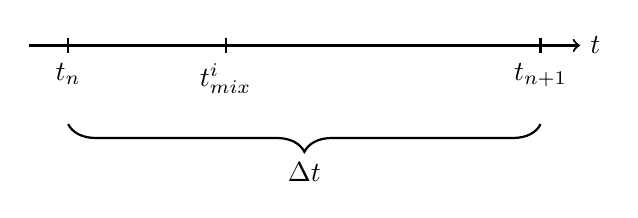
\begin{tikzpicture}[thick]

% Main timeline
\draw[->] (-0.5,0) -- (6.5,0) node[right] {$t$}; % Timeline with axis label

% Time points
\foreach \x/\label in {0/{$t_n$}, 2/{$t^i_\text{mix}$}, 6/{$t_{n+1}$}} {
    \draw (\x,0.1) -- (\x,-0.1) node[below] {\label};
}

% Braces for interval
\draw[decorate,decoration={brace,amplitude=10pt,mirror}] (0,-1) -- (6,-1) node[midway,below=10pt] {$\Delta t$};


\end{tikzpicture}
\end{figure}

arba kitaip sakant išmaišymas įvyks laiko žingsniu $t_n$, jei:

\begin{align}
    \vert t_n - t^i_\text{mix} \vert < \frac{1}{2}\Delta t \label{mix-inequality}
\end{align}

\paragraph{Nedeterministinis maišymas}

Maišymas praktikoje yra chaotiškas procesas, todėl sudarydami kompiuterinį modelį turime į tai atsižvelgti. Maišymą modeliuosime kaip reakcijos erdvės sričių atsitiktinį išdėstymą. Pradinė erdvę $\Omega$ padalinsime į mažesnes, nepersidengiančias, vienodas kvadratines sritis $\Omega_i$:

\begin{figure}[!h]
\centering
\caption{Padalinta reakcijos erdvė $\Omega$}
\label{split-reaction-space}

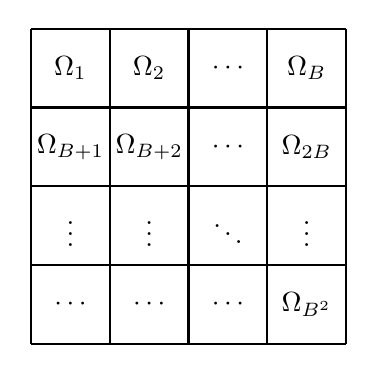
\begin{tikzpicture}
% Draw grid
\draw[thick] (0,0) grid (4,4);

% Row 1
\node at (0.5, 3.5) {$\Omega_1$};
\node at (1.5, 3.5) {$\Omega_2$};
\node at (2.5, 3.5) {$\cdots$};
\node at (3.5, 3.5) {$\Omega_B$};

% Row 2
\node at (0.5, 2.5) {$\Omega_{B + 1}$};
\node at (1.5, 2.5) {$\Omega_{B + 2}$};
\node at (2.5, 2.5) {$\cdots$};
\node at (3.5, 2.5) {$\Omega_{2B}$};

% Row 3
\node at (0.5, 1.5) {$\vdots$};
\node at (1.5, 1.5) {$\vdots$};
\node at (2.5, 1.5) {$\ddots$};
\node at (3.5, 1.5) {$\vdots$};

% Row 4
\node at (0.5, 0.5) {$\cdots$};
\node at (1.5, 0.5) {$\cdots$};
\node at (2.5, 0.5) {$\cdots$};
\node at (3.5, 0.5) {$\Omega_{B^2}$};
\end{tikzpicture}
\end{figure}

Tada sugeneruosime atsitiktinę $B^2$-permutaciją $\sigma: \{ 1, 2, \dots, B^2 \} \to \{ 1, 2, \dots, B^2 \} $ ir $B^2$ atsitiktinių kampų $\theta_i \in \{0, \frac{\pi}{2}, \pi, \frac{3\pi}{2}\}$. Kiekviena iš sričių $\Omega_i$ keliauja į poziciją, kurioje yra sritis $\Omega_{\sigma(i)}$, tačiau pasukta kampu $\theta_i$. Čia, kaip kompiuterinio modelio vartotojai, mes galime pasirinkti sričių kiekio parametrą $B\in\mathbb{N}$, tačiau reikia užtikrinti, kad diskrečių erdvės taškų kiekiai $N, M$ atitinkamomis ašimis būtų dalomi iš $B$. 

Atlikus tokį erdvės sudalinimą, gali atsitikti taip, kad kai kurių sričių $\Omega_i$ kaimynės bus tos pačios medžiagos arba atsisukusios į srities $\Omega$ išorę ir dėl to ties jų sandūra reakcija nevyks. Po išmaišymo tai gali pasikeisti ir galime daryti spėjimą, kad turėtume matyti staigų reakcijos greičio padidėjimą. 

% \paragraph{Neskylančios mikrodalelės}

% Norint atkartoti praktikoje pastebimą faktą, kad išmaišymo metu reagentų mikrodalelės nėra smulkinamos, modeliuodami medžiagų maišymą apsiribojime, kad 


% aprasyti kaip tas maisymas atrodo is tikro ir kaip skiriasi nuo modelio

% matematinis modelis maisymui
% stop salyga

\subsection{Reakcijos stabdymo sąlyga}

Pristatyti kompiuterinio modelio rezultatai rodo, kad vykstant reakcijai, reagentų kiekis erdvėje artėja prie 0, tačiau niekad jo nepasiekia. Tai būdinga ir realybėje vykstančioms reakcijoms, dėl šios priežasties kompiuterinio modelio darbą stabdysime, kai sureaguos $\eta_\text{stop}\%$ pradinių medžiagų kiekio. Matematiškai reakcijos stabdymo laiką $t_\text{stop}$ galime apibrėžti taip:

\begin{align}
    q(t_\text{stop})=\left(1-\frac{\eta_\text{stop}}{100}\right)q(0),\quad \eta_\text{stop}\in[0, 100)
\end{align}

\newpage
\subsection{Maišymo procesu papildytos programos rezultatų analizė}

\begin{figure}[h!]
\centering
\caption{Kompiuterinio modelio, papildyto išmaišymo procesu, rezultato pavyzdys. Čia $\eta_\text{stop} = 97$, $t^1_\text{mix} = 1h$, $B = 2$, $D = 28\times 10^{-6} \frac{\mu m^2}{s}$, $W = \sqrt[3]{10}\mu m$, $H = \sqrt[3]{10}\mu m$, $k = 0$, $c_0 = 10^{-6} \frac{g}{\mu m^3}$, $\Delta x = \Delta y = \frac{\sqrt[3]{10}}{79} \mu m$ }
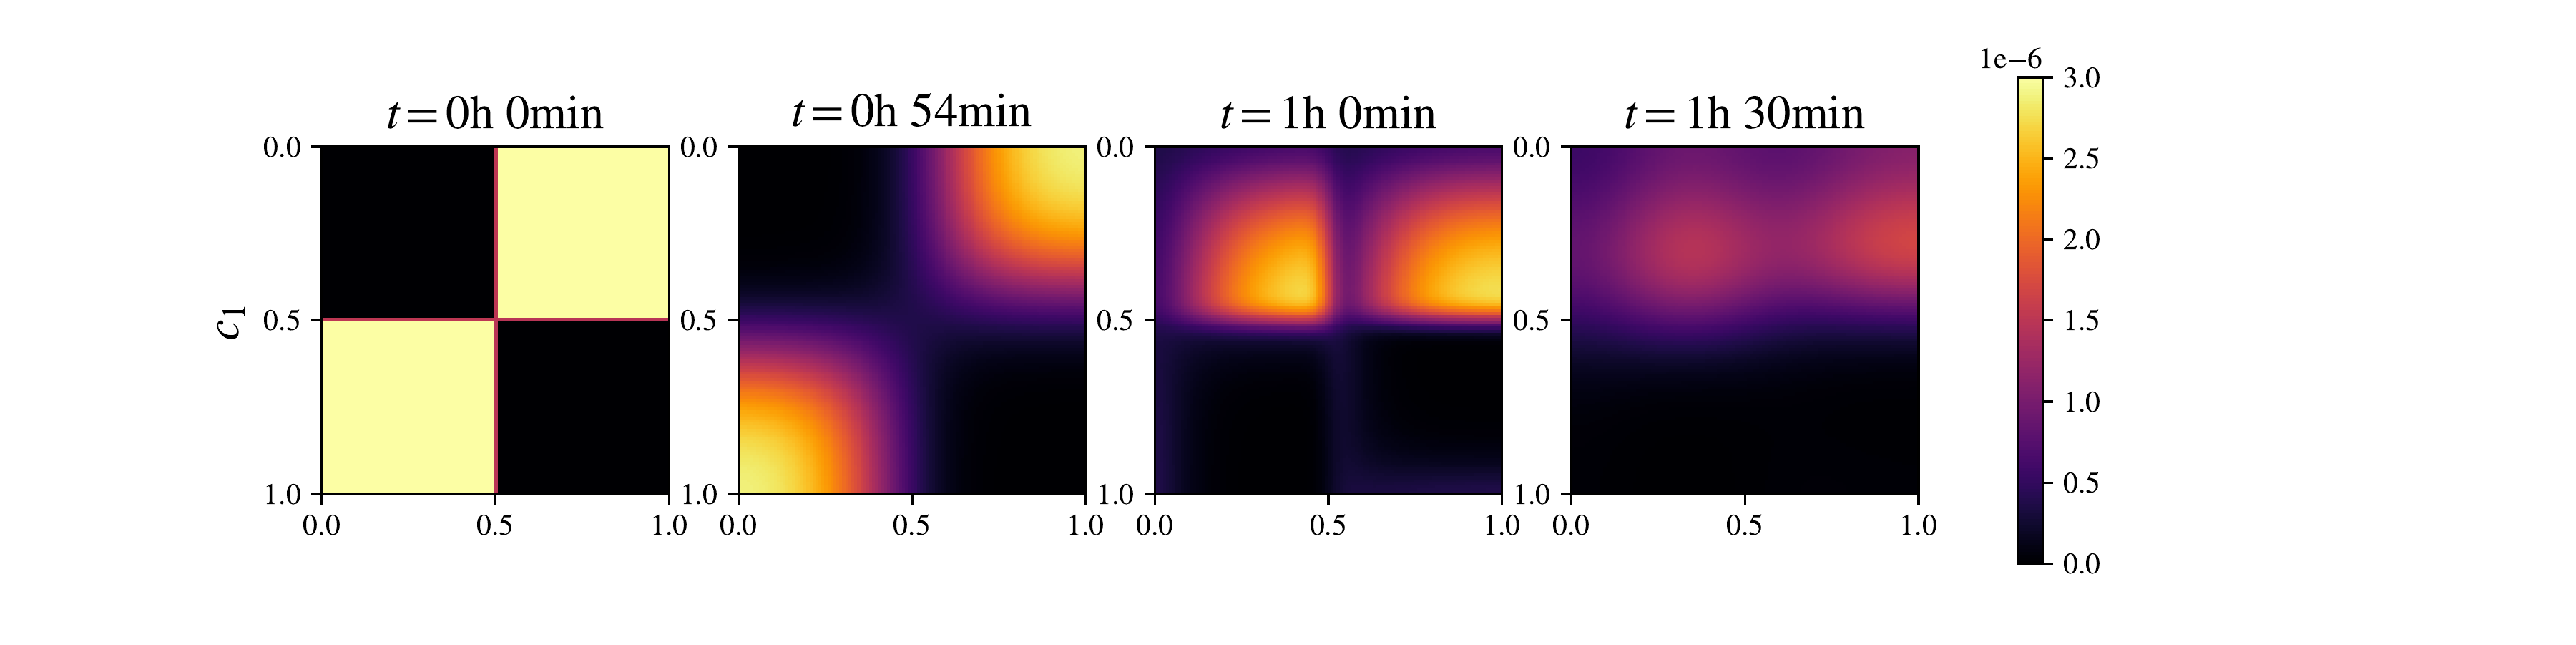
\includegraphics[width=\textwidth]{../paper/assets/random-mix-example-c0-1.png} \\
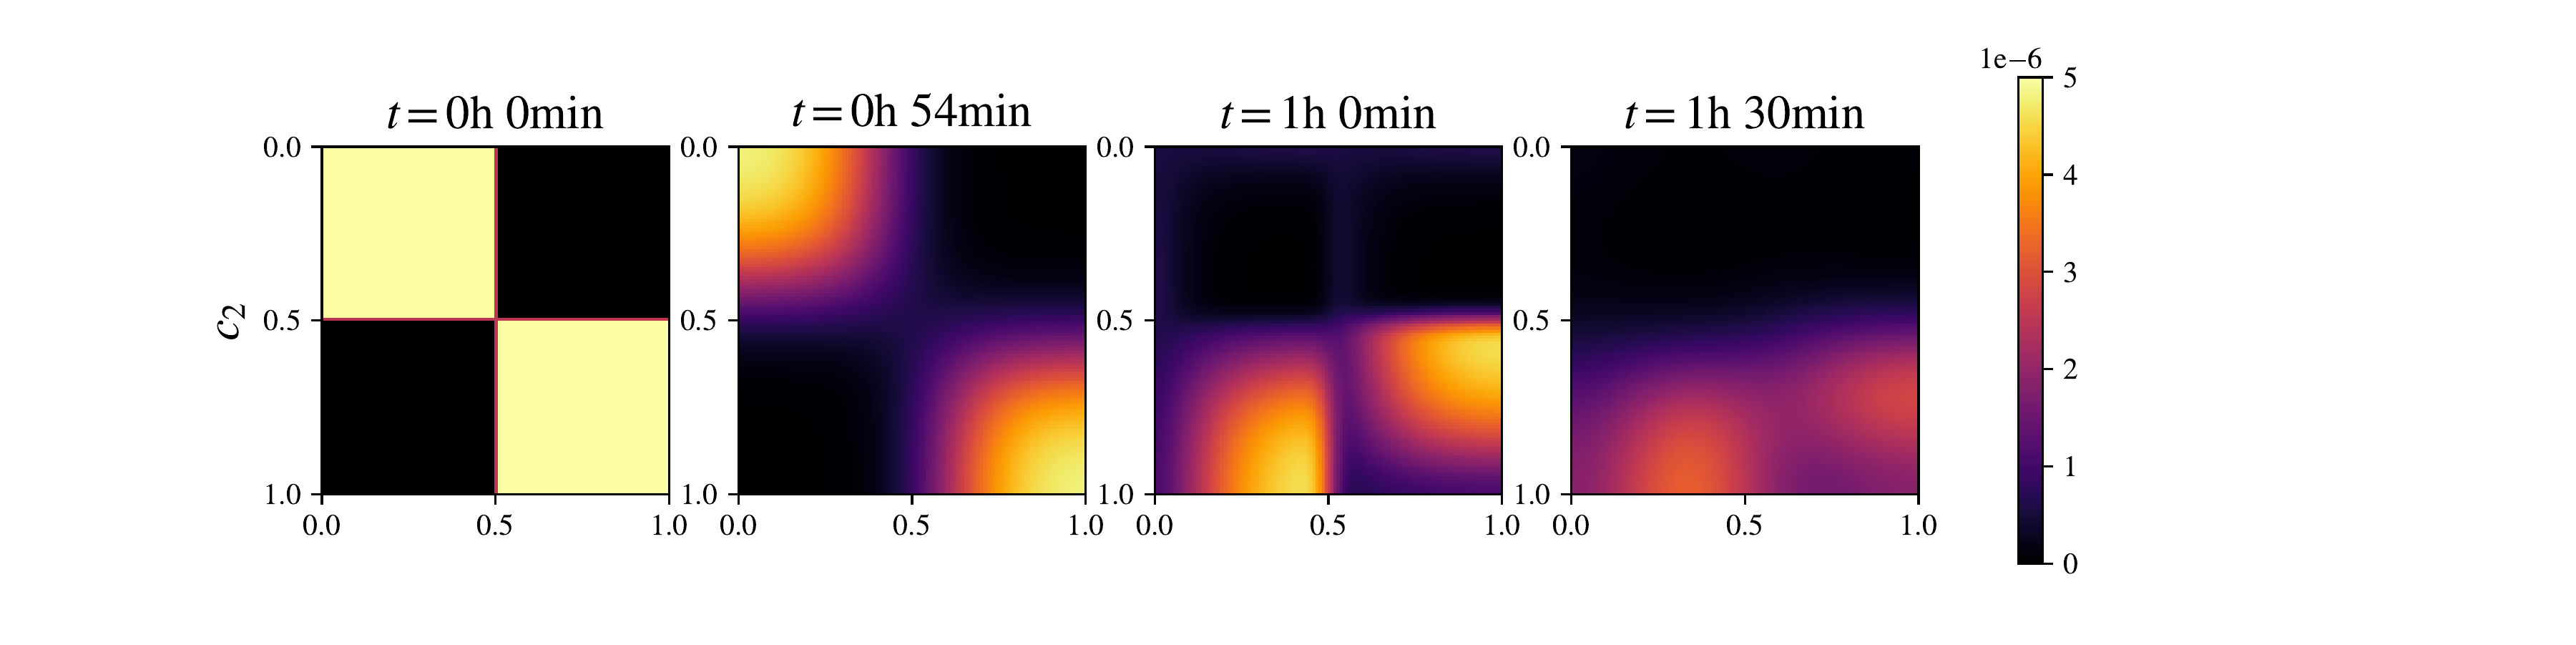
\includegraphics[width=\textwidth]{../paper/assets/random-mix-example-c1-1.png} \\
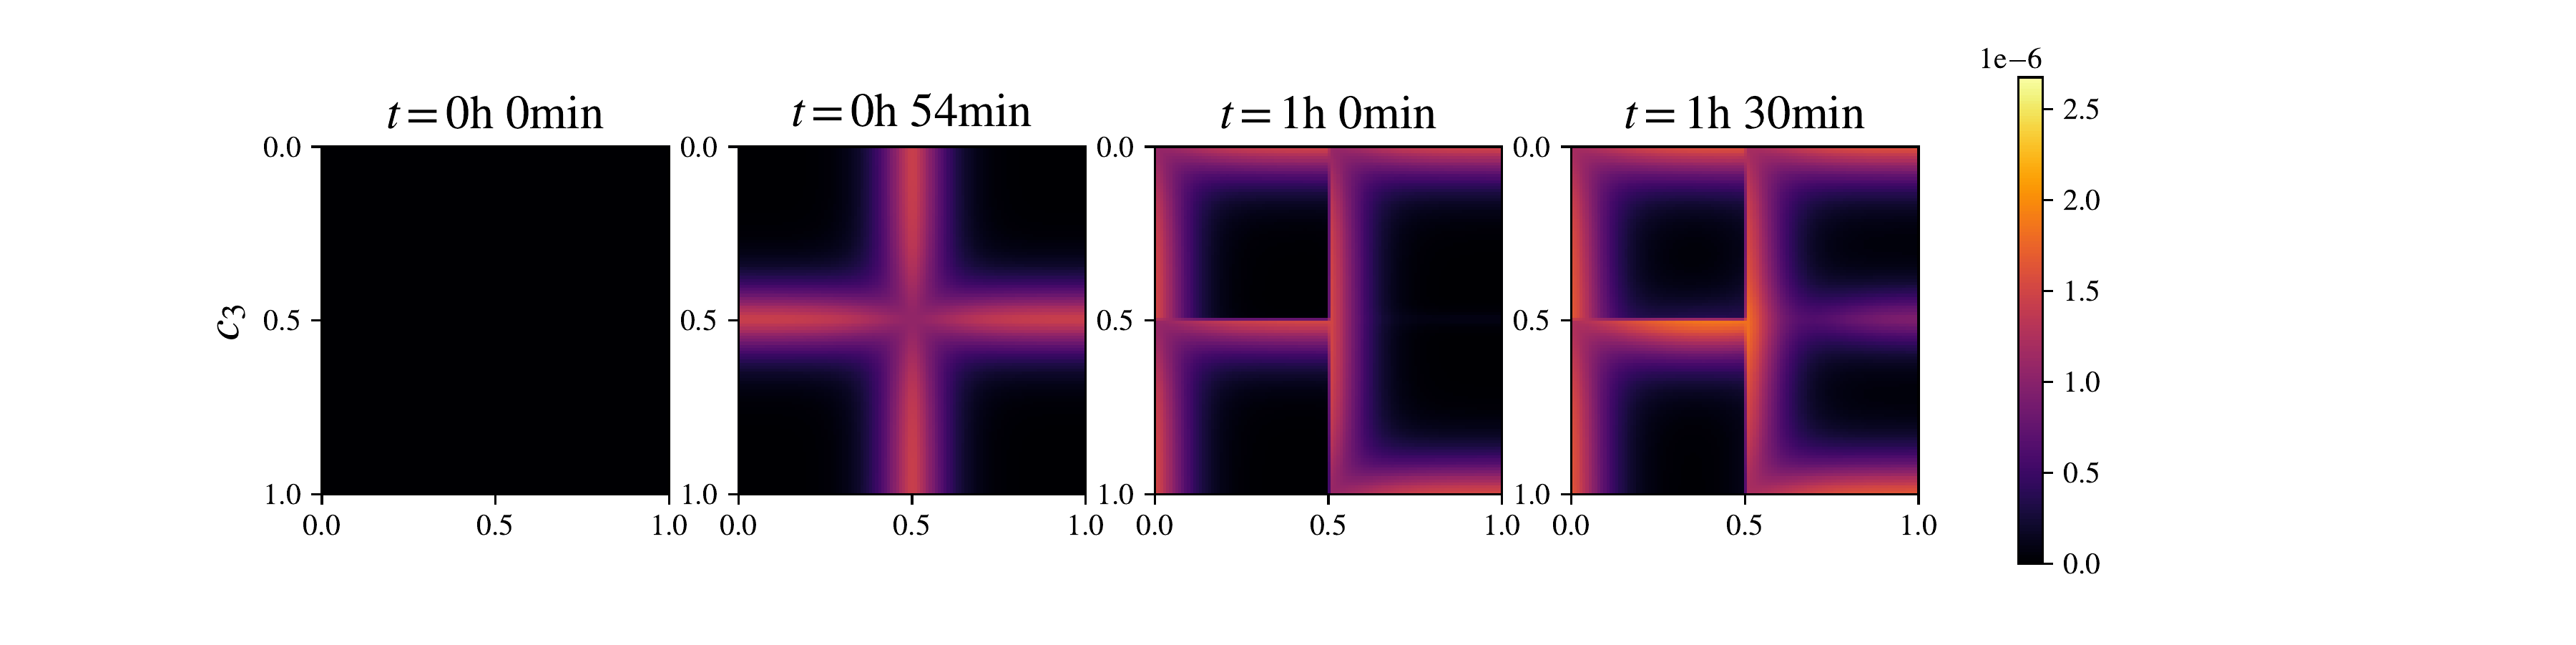
\includegraphics[width=\textwidth]{../paper/assets/random-mix-example-c2-1.png}
\label{mix-example}
\end{figure}

\ref{mix-example}-ame pavyzdyje matome kaip atrodo reakcijos eiga, kada vyksta išmaišymas. Šiuo atveju išmaišymas vyko laiku $t=1h$. Trečias stulpelis vaizduoja reakcijos erdvę ką tik po išmaišymo proceso, kada visos keturios sritys $\Omega_i$ yra atsitiktinai pasukamos ir sumaišomos. Kadangi nuo išmaišymo praejo labai mažai laiko, medžiagos nespėjo sureaguoti ir dėl to matome didelio kontrasto artefaktus ties kai kuriomis išmaišytų sričių kraštinėmis. Čia galime pastebėti tam tikrą problemą su atsitiktiniu išmaišymu - šiuo atveju, po išmaišymo, nesusidūrė prieš tai dar nesureagavusios dalelių kraštinės, todėl reakcijos greičiui šis procesas neturėjo beveik jokios įtakos. Tai gana akivaizdžiai matosi jei pažiūrėtume į medžiagos kiekio grafiką.

\newpage

\begin{figure}[h!]
    \centering
    \caption{Kompiuterinio modelio rezultatų palyginimas su ir be maišymo proceso. Čia $\eta_\text{stop} = 97$, $B = 2$, $D = 28\times 10^{-6} \frac{\mu m^2}{s}$, $W = \sqrt[3]{10}\mu m$, $H = \sqrt[3]{10}\mu m$, $k = 0$, $c_0 = 10^{-6} \frac{g}{\mu m^3}$, $\Delta x = \Delta y = \frac{\sqrt[3]{10}}{79} \mu m$ }
    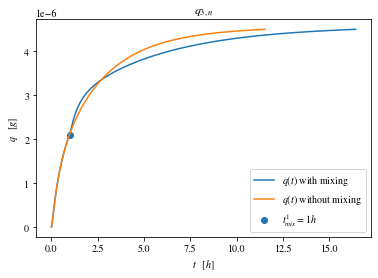
\includegraphics[width=0.5\textwidth]{../paper/assets/bad-mix-qnt-compare.png}
    \label{bad-mix-qnt-example}
\end{figure}

\ref{bad-mix-qnt-example}-ame pavyzdyje puikiai matosi, kad išmaišymas nepagreitino reakcijos, o ją sulėtino. Praktiniuose eksperimentuose taip niekad nenutinka todėl, kad mikrodalelių skaičius yra pakankamai didelis ir toks atvejis tampa beveik neįmanomas. Šiuo atveju galėtume pakeisti 


